 \documentclass{beamer}

\usepackage[utf8]{inputenc}
\usepackage[russian]{babel}
\usepackage{cmap}

\mode<presentation> {
\usetheme{Madrid}
\setbeamertemplate{caption}[numbered]
}

\usepackage{graphicx} % Allows including images
\usepackage{booktabs} % Allows the use of \toprule, \midrule and \bottomrule in tables

\title[Технологии разработки ПО]{Kormushka:\\финансовый менеджмент малого коллектива}

\author{Black team.}
\institute[СПб ПУ]
{
Санкт-Петербургский государственный политехнический университет \\
\medskip
\textit{https://github.com/SemenMartynov/kormushka}
}
\date{\today}

\begin{document}

\begin{frame}
\titlepage
\end{frame}

\begin{frame}
\frametitle{Содержание}
\tableofcontents
\end{frame}

%------------------------------------------------
\section{Команда}
%------------------------------------------------

\begin{frame}
\frametitle{Команда: распределение ролей}

\begin{itemize}
\item Мяснов Александр (Client),
\bigskip
\bigskip
\item Дедков Сергей (Project Manager),
\medskip
\item Антон Абрамов (Lead programmer),
\medskip
\item Влад Бусаров (Software Engineer),
\medskip
\item Николай Патраков (Software Engineer),
\medskip
\item Семён Мартынов (Quality Assurance).
\end{itemize}

\end{frame}

%------------------------------------------------
\section{Постановка задачи}
%------------------------------------------------

\begin{frame}
\frametitle{Постановка задачи}

Приложение для взаиморасчётов в не большом коллективе.

\begin{itemize}
\item Накопление данных о тратах
\item Подсчёт вклада каждого участника группы
\item Формирование отчёта за какой-то период
\item Создание плана взаиморасчётов
\end{itemize}

\end{frame}

%------------------------------------------------
\section{Процессы и инструменты}
%------------------------------------------------

\begin{frame}
\frametitle{Выбор стека технологий}

\begin{columns}[t]
\column{.45\textwidth} % Left column and width
Язык:
\begin{itemize}
\item PHP
\item Python
\item Ruby
\item JavaEE
\item C\#
\item СPP
\end{itemize}

\column{.5\textwidth} % Right column and width
БД:
\begin{itemize}
\item MySQL
\item SQLite
\item MS SQL
\item NoSQL
\end{itemize}
\end{columns}

\end{frame}

%------------------------------------------------

\begin{frame}
\frametitle{Выбор лицензии}

\begin{block}{GNU General Public License}
Открытое лицензионное соглашение передачи программного обеспечения в общественную собственность
\end{block}
\bigskip
\begin{block}{MIT}
Лицензия свободного программного обеспечения разработанная Массачусетским технологическим институтом (MIT).
\end{block}

\end{frame}

%------------------------------------------------

\subsection{Хранение кода}

\begin{frame}
\frametitle{Хранение кода}

\begin{block}{GitHub}
Самый крупный веб-сервис для хостинга IT-проектов и их совместной разработки, основан на распределённой системе контроля версий Git.
\end{block}

Использование распределённой системы контроля версий позволяет работать с кодом даже когда нет интернета (актуально для некоторых членов нашей команды).

\begin{figure}
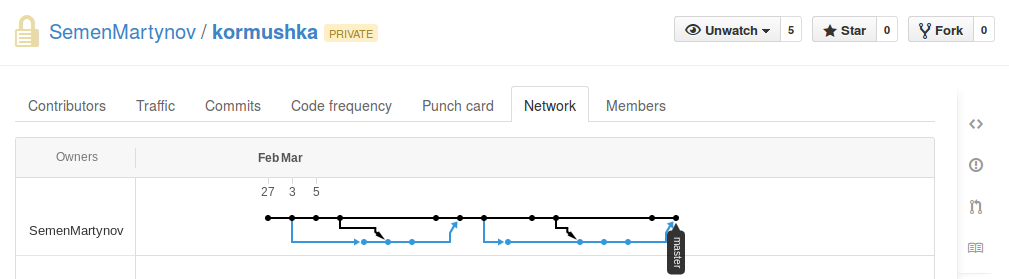
\includegraphics[scale=0.30]{res/r1_git}
\caption{Коммиты участников проекта в репозиторий}
\end{figure}

\end{frame}

%------------------------------------------------

\subsection{Управление задачами}

\begin{frame}
\frametitle{Управление задачами: milestones}

\begin{figure}
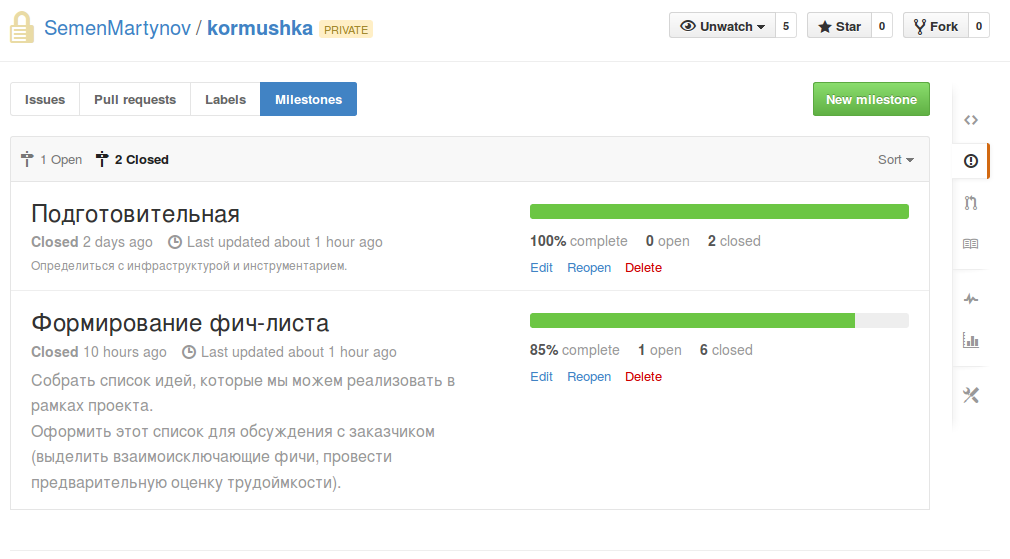
\includegraphics[scale=0.30]{res/r1_milestones}
\caption{Задачи группируются в milestones}
\end{figure}

\end{frame}

%------------------------------------------------

\begin{frame}
\frametitle{Управление задачами: issues}

\begin{figure}
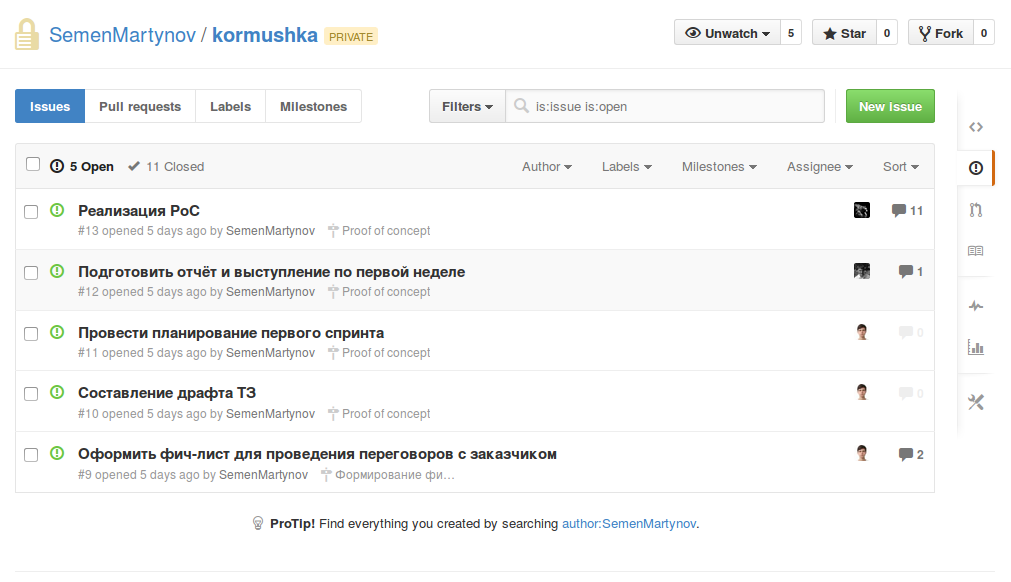
\includegraphics[scale=0.30]{res/r1_issues}
\caption{Все задачи обсуждаются и отслеживаются}
\end{figure}

\end{frame}

%------------------------------------------------


\subsection{Управление знаниями}

\begin{frame}
\frametitle{Управление знаниями}

\begin{figure}
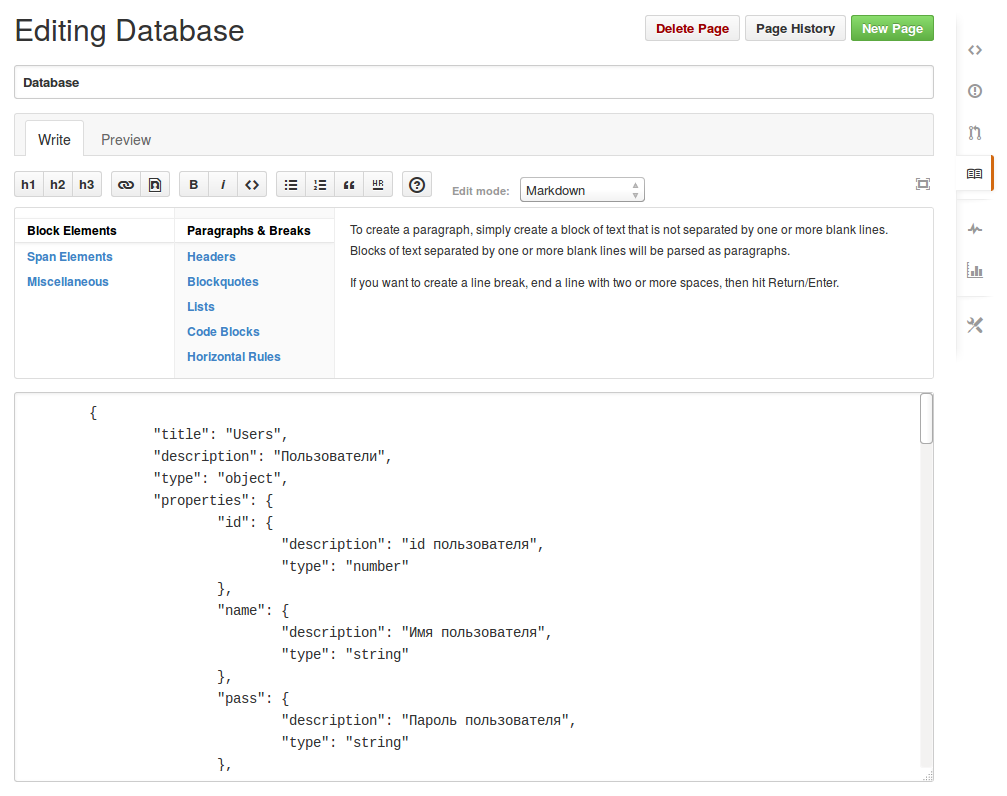
\includegraphics[scale=0.25]{res/r1_wiki}
\caption{Все ценные артефакты хранятся в wiki}
\end{figure}

\end{frame}

%------------------------------------------------
\section{Встреченные сложности}
%------------------------------------------------

\begin{frame}
\frametitle{Встреченные сложности}

Отсутствие достаточной функциональной спецификации!
\bigskip
\bigskip
Без чёткой спецификации невозможно провести правильную декомпозицию задач и планирование архитектуры!
\bigskip
\bigskip
На данный момент была проведена одна бриф-встреча с заказчиком.
\end{frame}


%------------------------------------------------
\section{Демонстрация результатов}
%------------------------------------------------

\begin{frame}
\frametitle{Демонстрация достигнутых результатов}

\begin{figure}
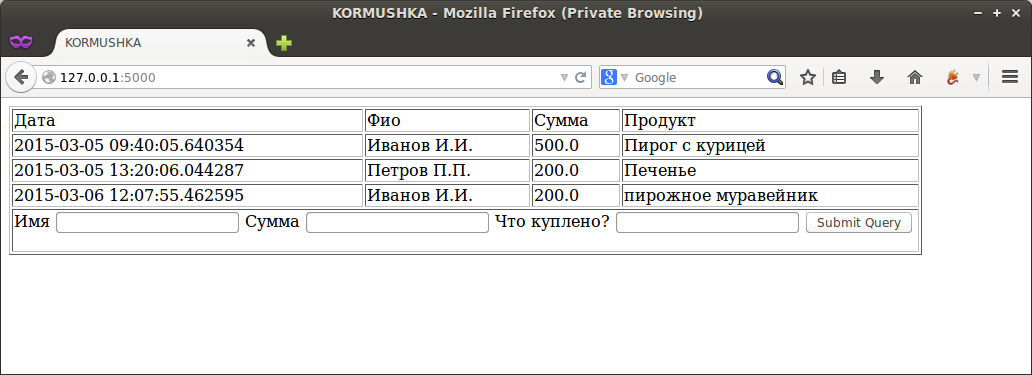
\includegraphics[scale=0.30]{res/r1_PoC}
\caption{PoC: Сбор и хранение информации сервером, написанном на Python}
\end{figure}

\end{frame}

%------------------------------------------------
\section{Цели первого спринта}
%------------------------------------------------

\begin{frame}
\frametitle{План первого спринта}

К концу первого спринта мы достигнем следующих результатов:
\medskip
\begin{itemize}
\item Составим и согласуем с заказчиком техническое задание
\medskip
\item Сформируем и начнём отслеживание набора метрик для оценки проекта
\medskip
\item Подготовим инфраструктуру для Continuous integration
\medskip
\item Сформируем alpha-версию продукта
\medskip
\item Развернём продукт на публично доступном сервере
\end{itemize}

\end{frame}

%------------------------------------------------
\section{Вопросы}
%------------------------------------------------

\begin{frame}
\Huge{\centerline{Вопросы?}}
\end{frame}

%----------------------------------------------------------------------------------------

\end{document} 
